\section{Diskussion}
\label{sec:Diskussion}

Aus den Werten der Dichten $\rho$ der beiden Stäbe
\begin{align*}
    \overline{\rho_\square} &= \SI{8902.66 (5.62)}{\kilo\gram\per\meter^3}, \\
    \overline{\rho_\bigcirc} &= \SI{8862.79 (12.37)}{\kilo\gram\per\meter^3}, \\
\end{align*}
wird darauf geschlossen, dass das Material des Stabes Kupfer ist ($\rho_{\text{lit}} = \SI{8920}{\kilo\gram\per\meter^3}$).
Der Literaturwert für das Elastizitätsmodul von Kupfer lautet nach \cite{czichos}
\begin{align*}
    E_{\text{lit}} = \SI{125e9}{\Pa}.
\end{align*}
Aus dem Versuch wurden zwei Elastizitätsmodule, das eines eckigen und das eines runden Stabes bestimmt,
\begin{align*}
    \overline{E_{\square}} &= \SI{230(50)e9}{\Pa}, \\
    \overline{E_{\bigcirc}} &= \SI{149(4)e9}{\Pa}.
\end{align*}

\sloppy
Die Abweichungen der gemessenen Elastizitätsmodule betragen
$\upDelta_{\square} = 84 \%$ und $\upDelta_{\bigcirc} = 16.11 \%$.
Wird der zweite Wert für den Elastizitätsmodul des eckigen Stabes bei beidseitiger Auflage ($\SI{400(1500)e9}{\Pa}$)
aus dem Mittelwert gestrichen, da der Wert viel zu ungenau ist, so kommt ein neuer Mittelwert von
\begin{align*}
    \overline{E_{\square}} &= \SI{146(3.4)e9}{\Pa}
\end{align*}
heraus. Dieser Wert hat somit nur noch eine Abweichung von $\upDelta_{\square} = 14.38 \%$.
Für diesen Mittelwert und den des runden Stabes $\upDelta_{\bigcirc}$, lässt sich der Literaturwert 
des Elastizitätsmoduls für Kupfer verifizieren.

Grund für diese Ungenauigkeiten werden mitunter die Messuhren sein, die große Ungenauigkeiten verursachen können.
So schlugen die Zeiger bereits nach den kleinsten Erschütterungen aus, was das Messen erschwerte. 
Ein weiterer Grund für Abweichungen sind die Zustände der benutzten Kupferstäbe. So war der eckige Kupferstab laut der Messuhr
von großen Verbiegungen durchzogen, weshalb die Messwerte nicht linear erfolgten.
Bei der Messung der Auslenkungen bei beidseitigen Einspannungen wurden zwei Messuhren benutzt, eine rechts und eine links des Gewichtes.
Die linke Messuhr hat dabei keine den Werten der rechten Uhr kongruenten Werte gemessen, auch wenn dieselben Positionen vermessen wurden.
Auch die vergleichsweise nur geringen Auslenkungen der beiden Stäbe verursachen hohe Ungenauigkeiten, da nur in einem
kleinen Messbereich mit geringem Gewicht gemessen wird.
Eine andere mögliche Fehlerquelle könnte ein falscher Versuchsaufbau sein. So durfte bei beidseitiger Messung der Stabe nicht
eingespannt werden, wenn dies allerdings doch getan wurde, so sind die Werte ungenau.


\section{Anhang}
\label{sec:anhang}

\begin{figure}[H]
  \centering
  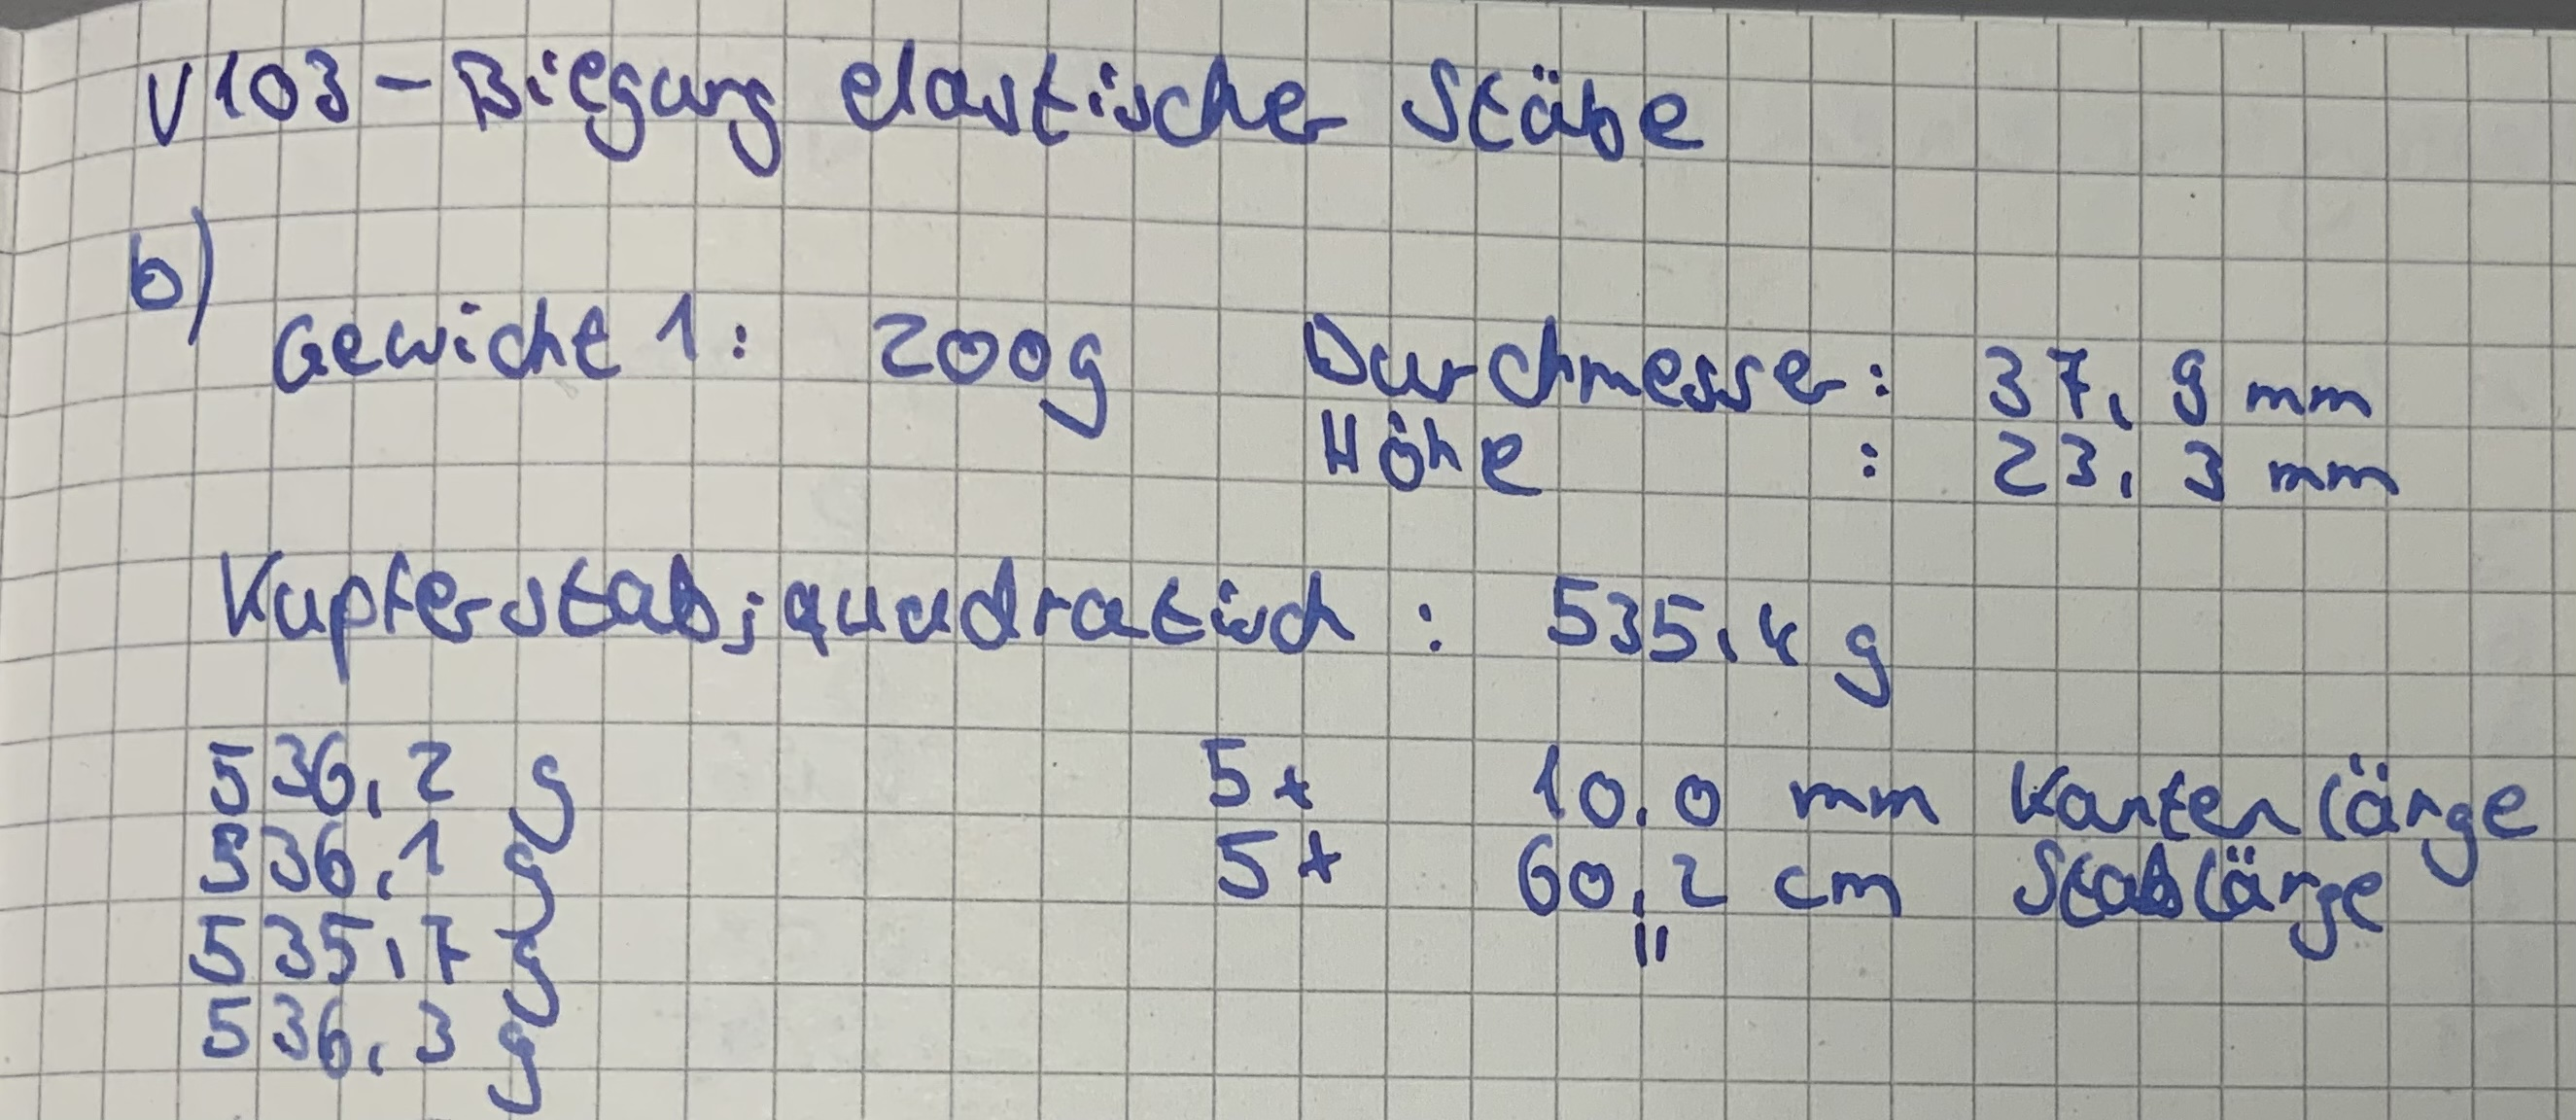
\includegraphics[width=0.75\textwidth]{Dateien/Bild1.jpeg}
  \caption{Originale Messdaten.}
  \label{fig:daten1}
\end{figure}

\begin{figure}[H]
    \centering
    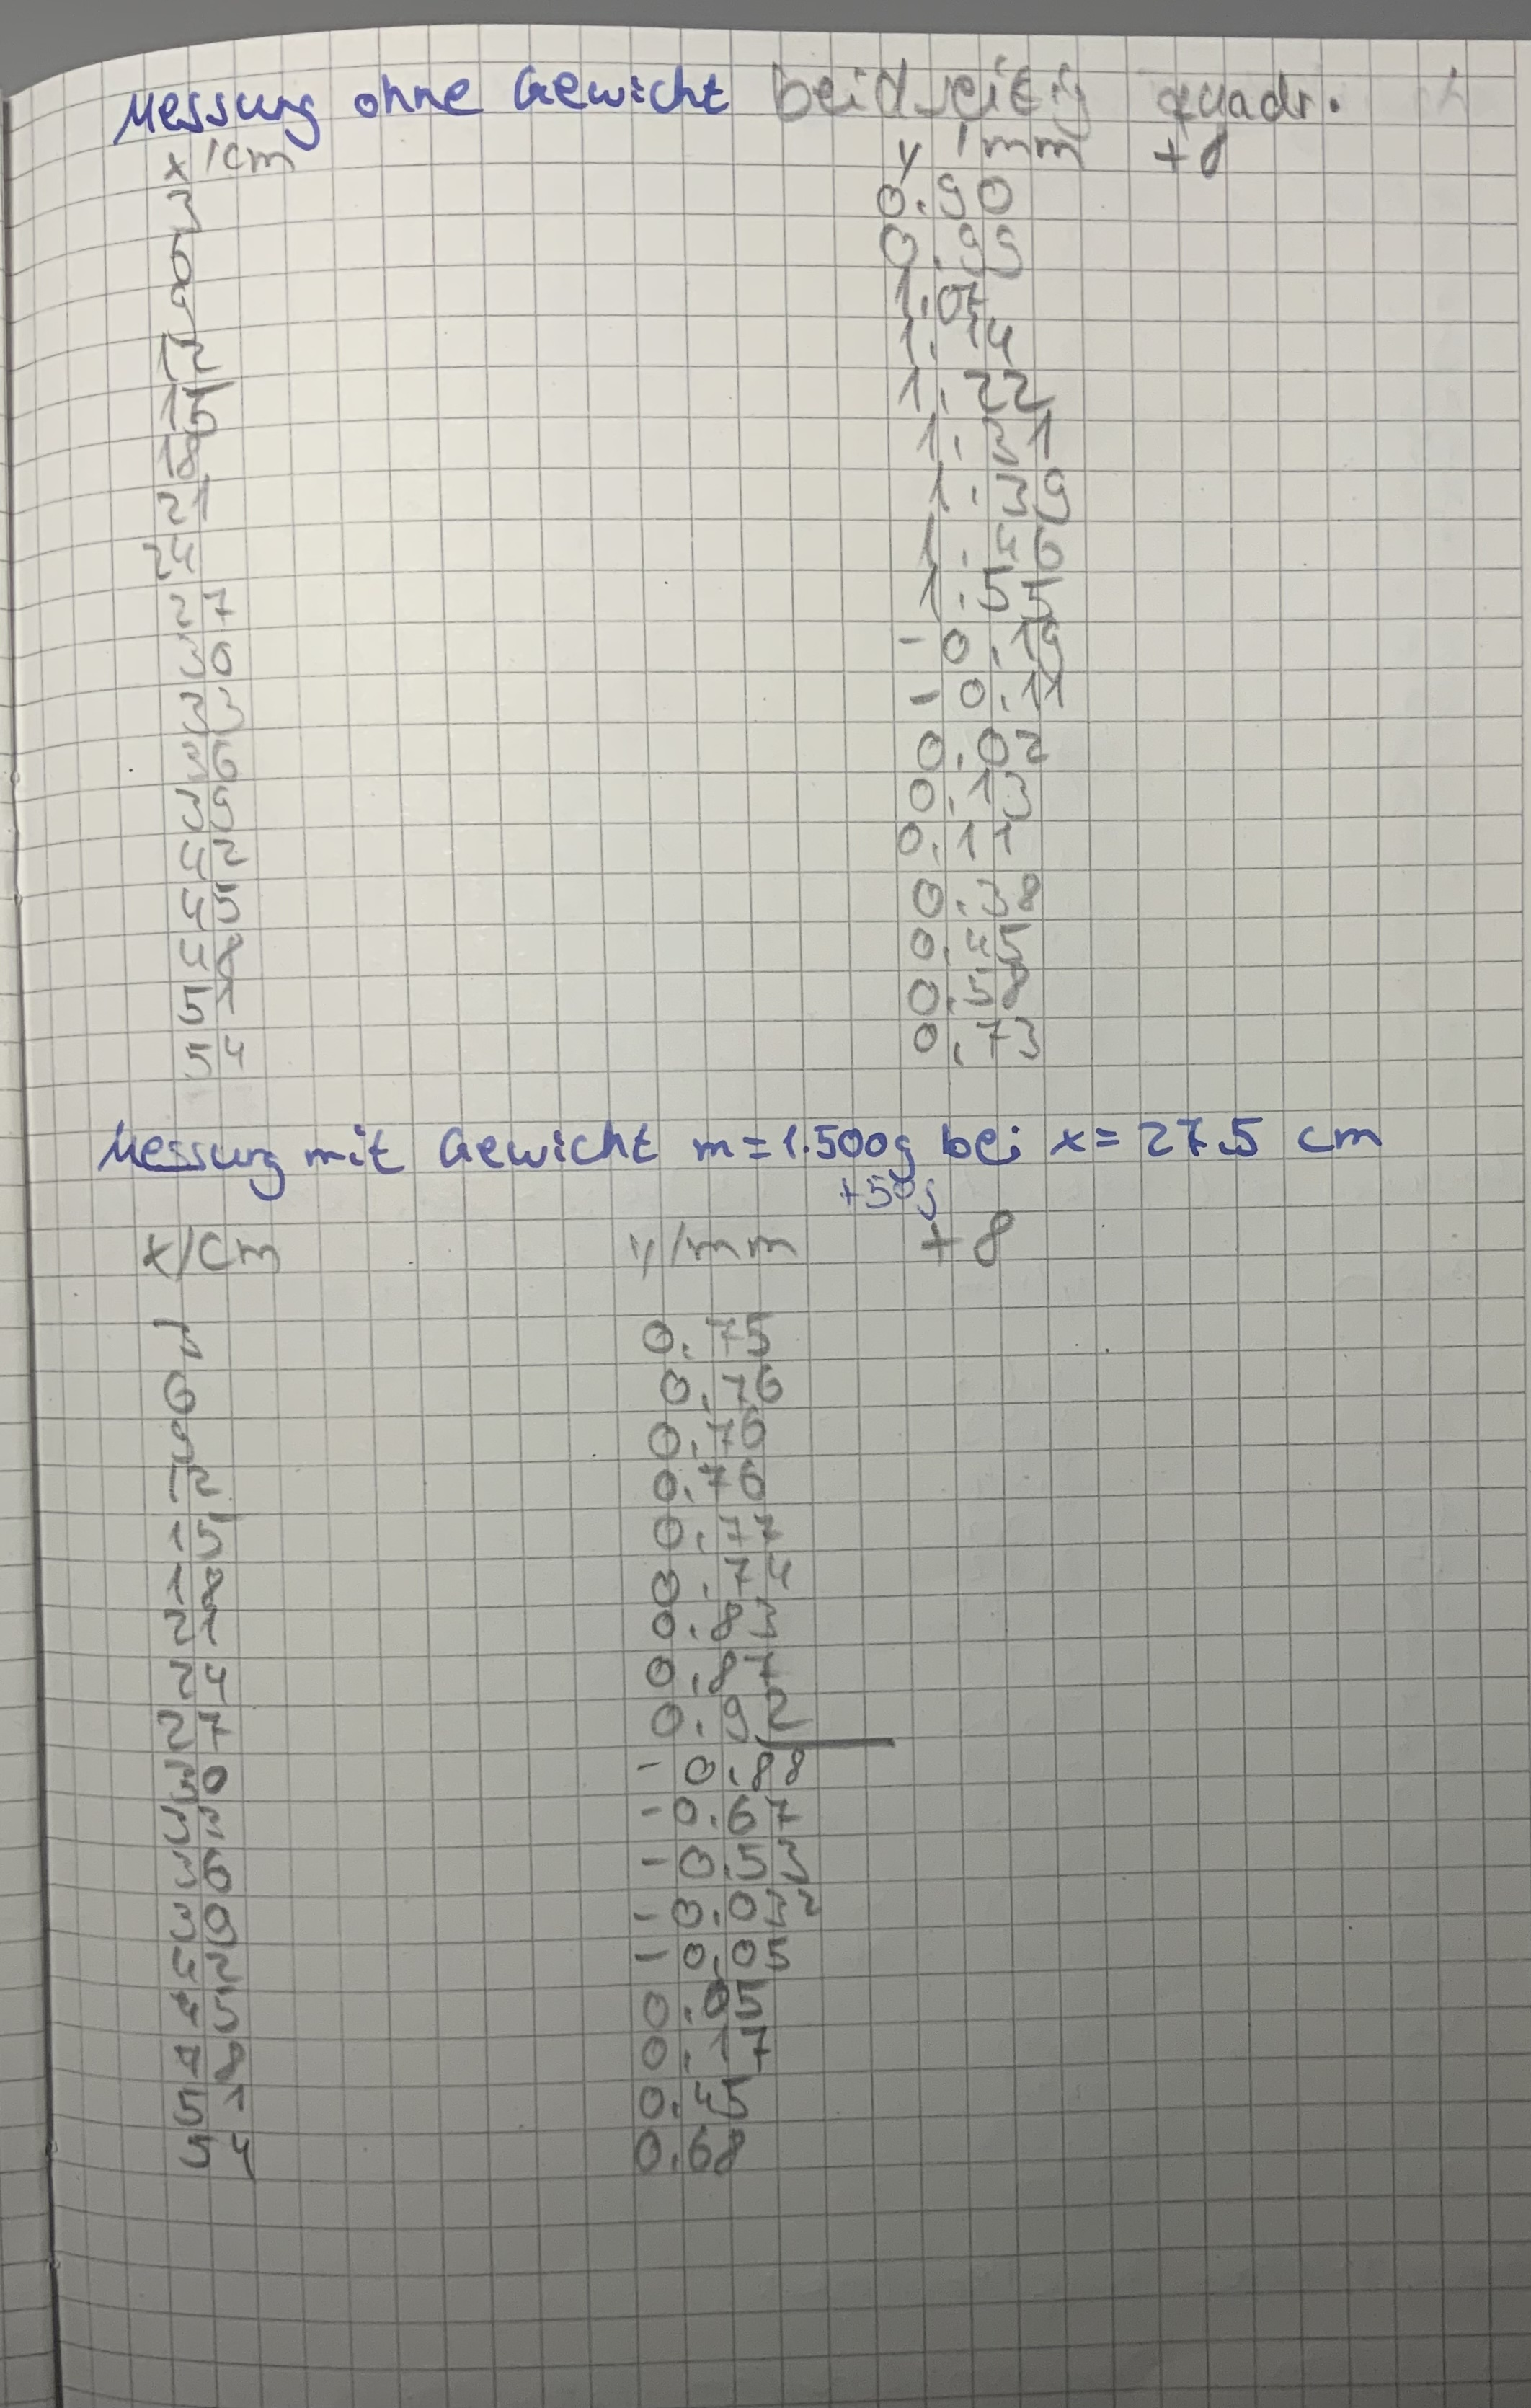
\includegraphics[width=0.75\textwidth]{Dateien/Bild2.jpeg}
    \caption{Originale Messdaten.}
    \label{fig:daten2}
\end{figure}

\begin{figure}[H]
    \centering
    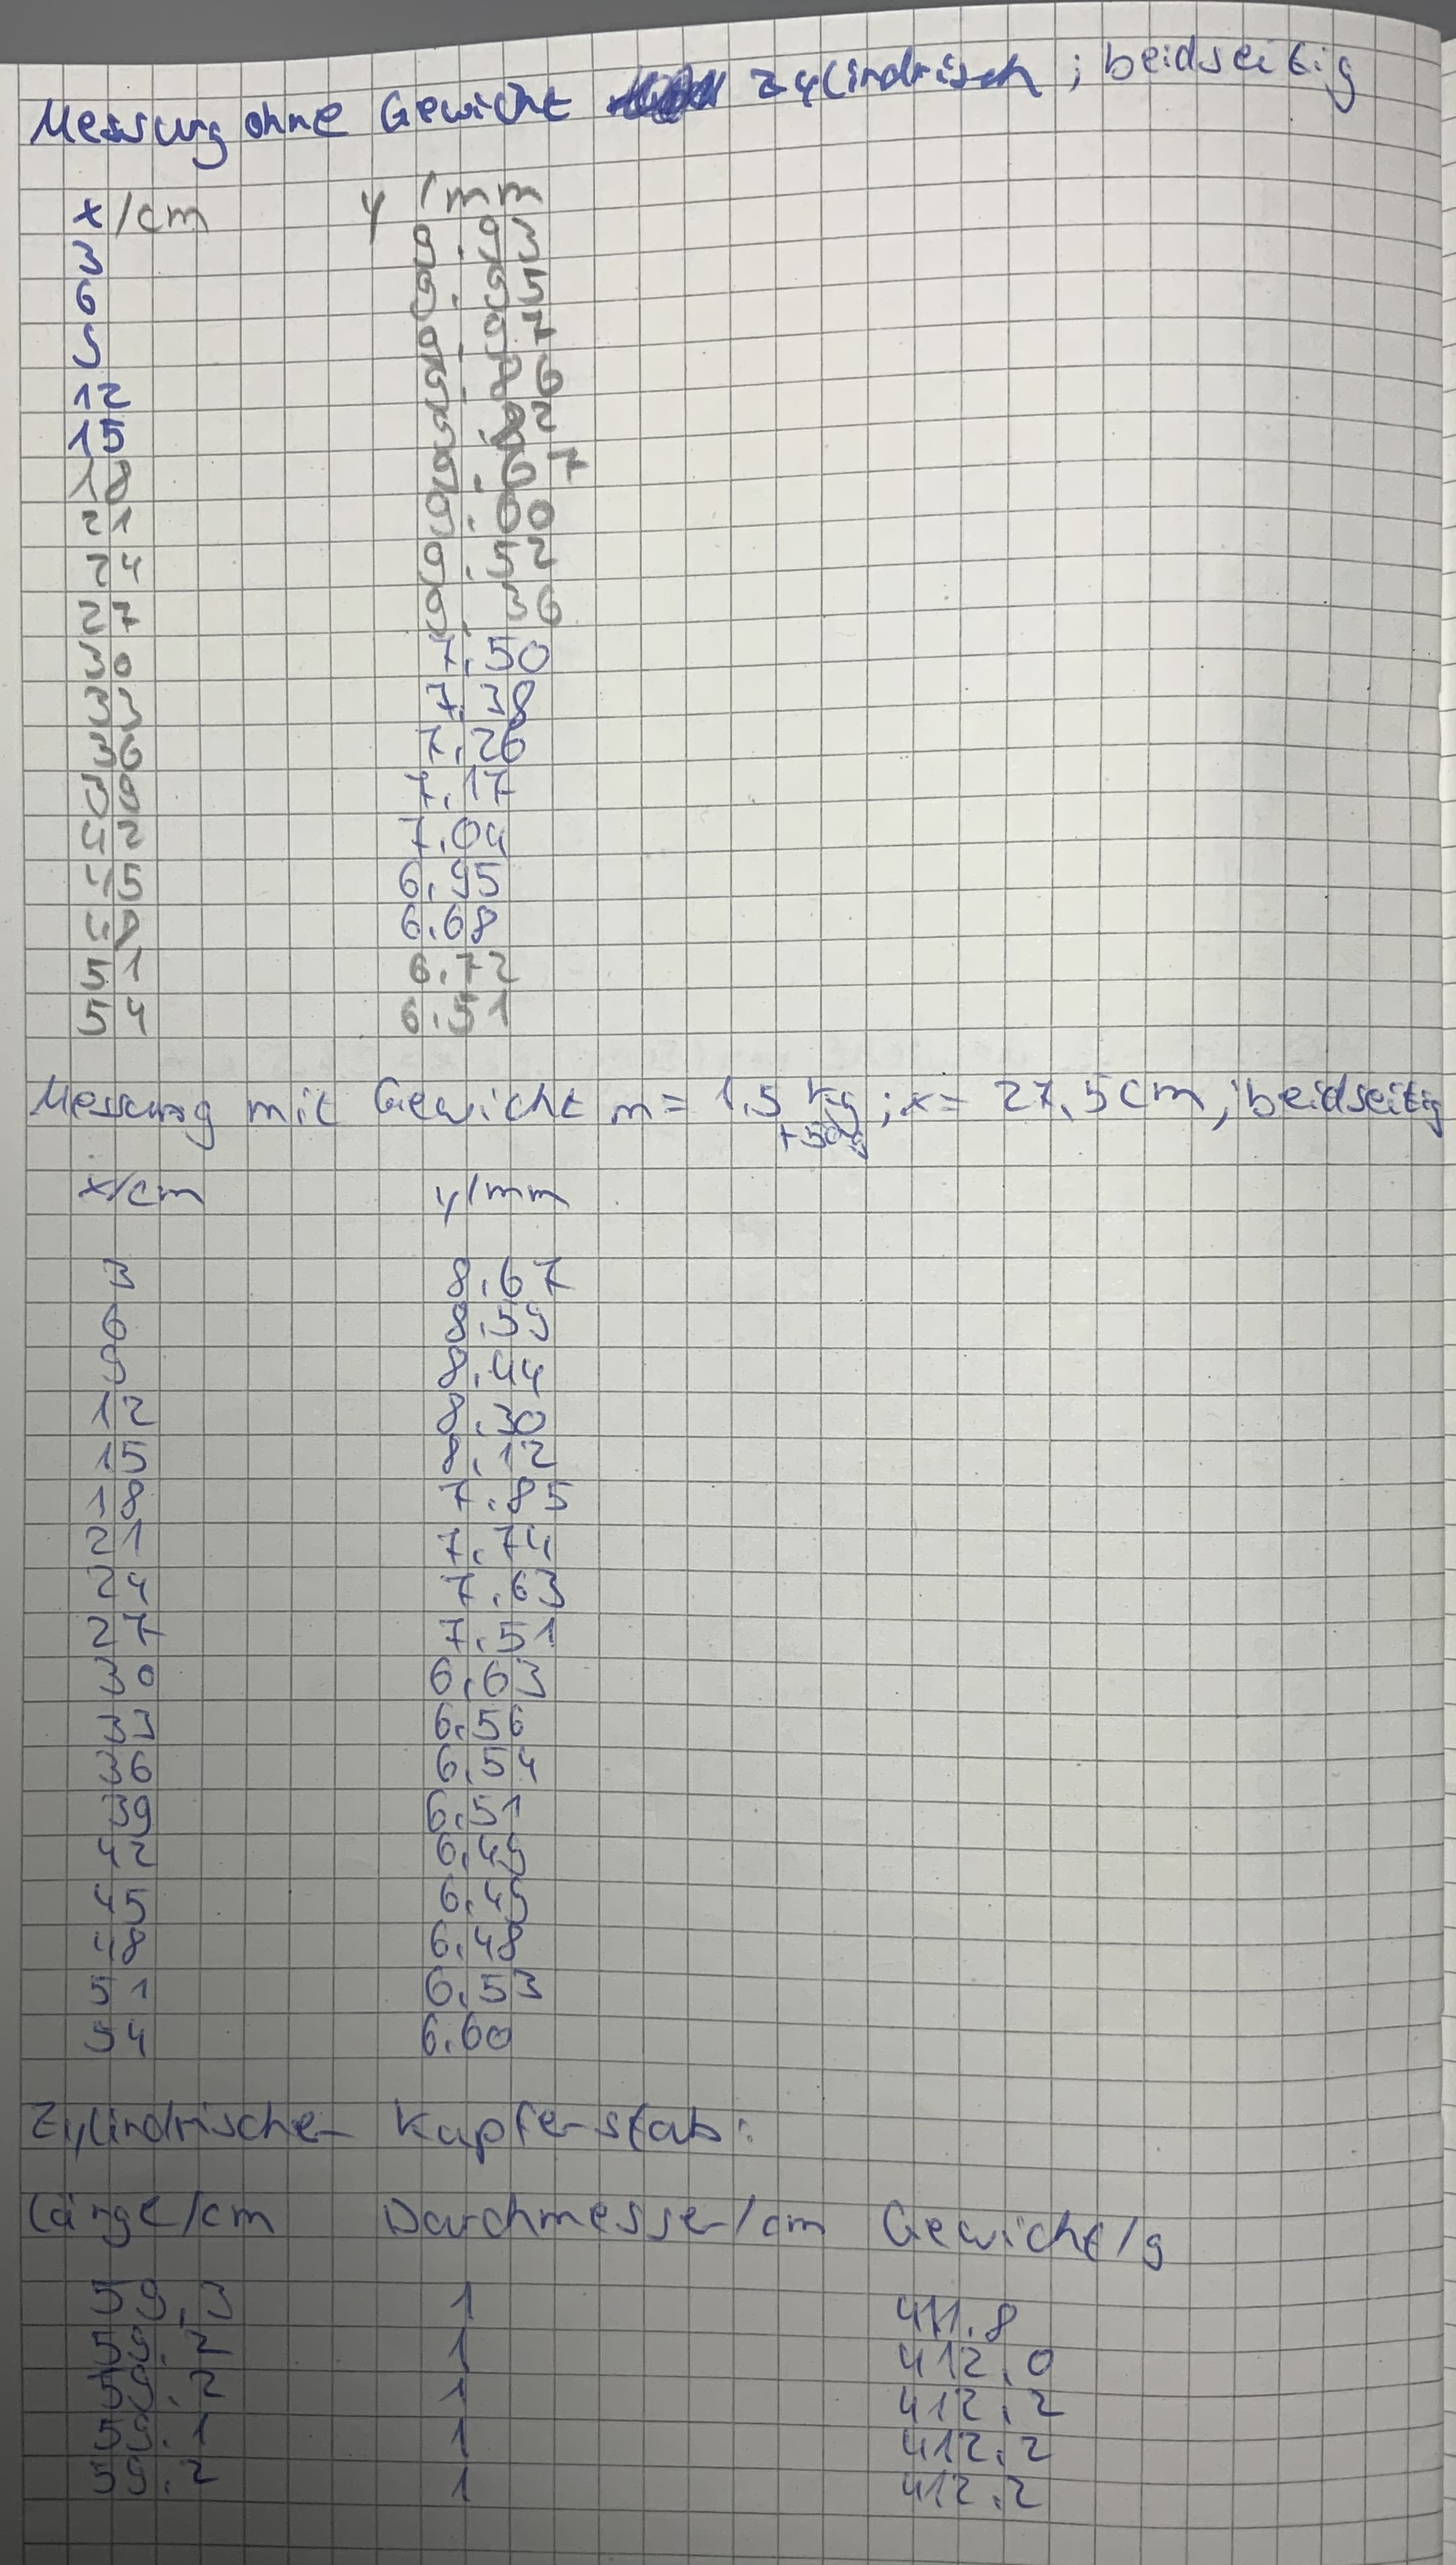
\includegraphics[width=0.75\textwidth]{Dateien/Bild3.jpeg}
    \caption{Originale Messdaten.}
    \label{fig:daten3}
\end{figure}

\begin{figure}[H]
    \centering
    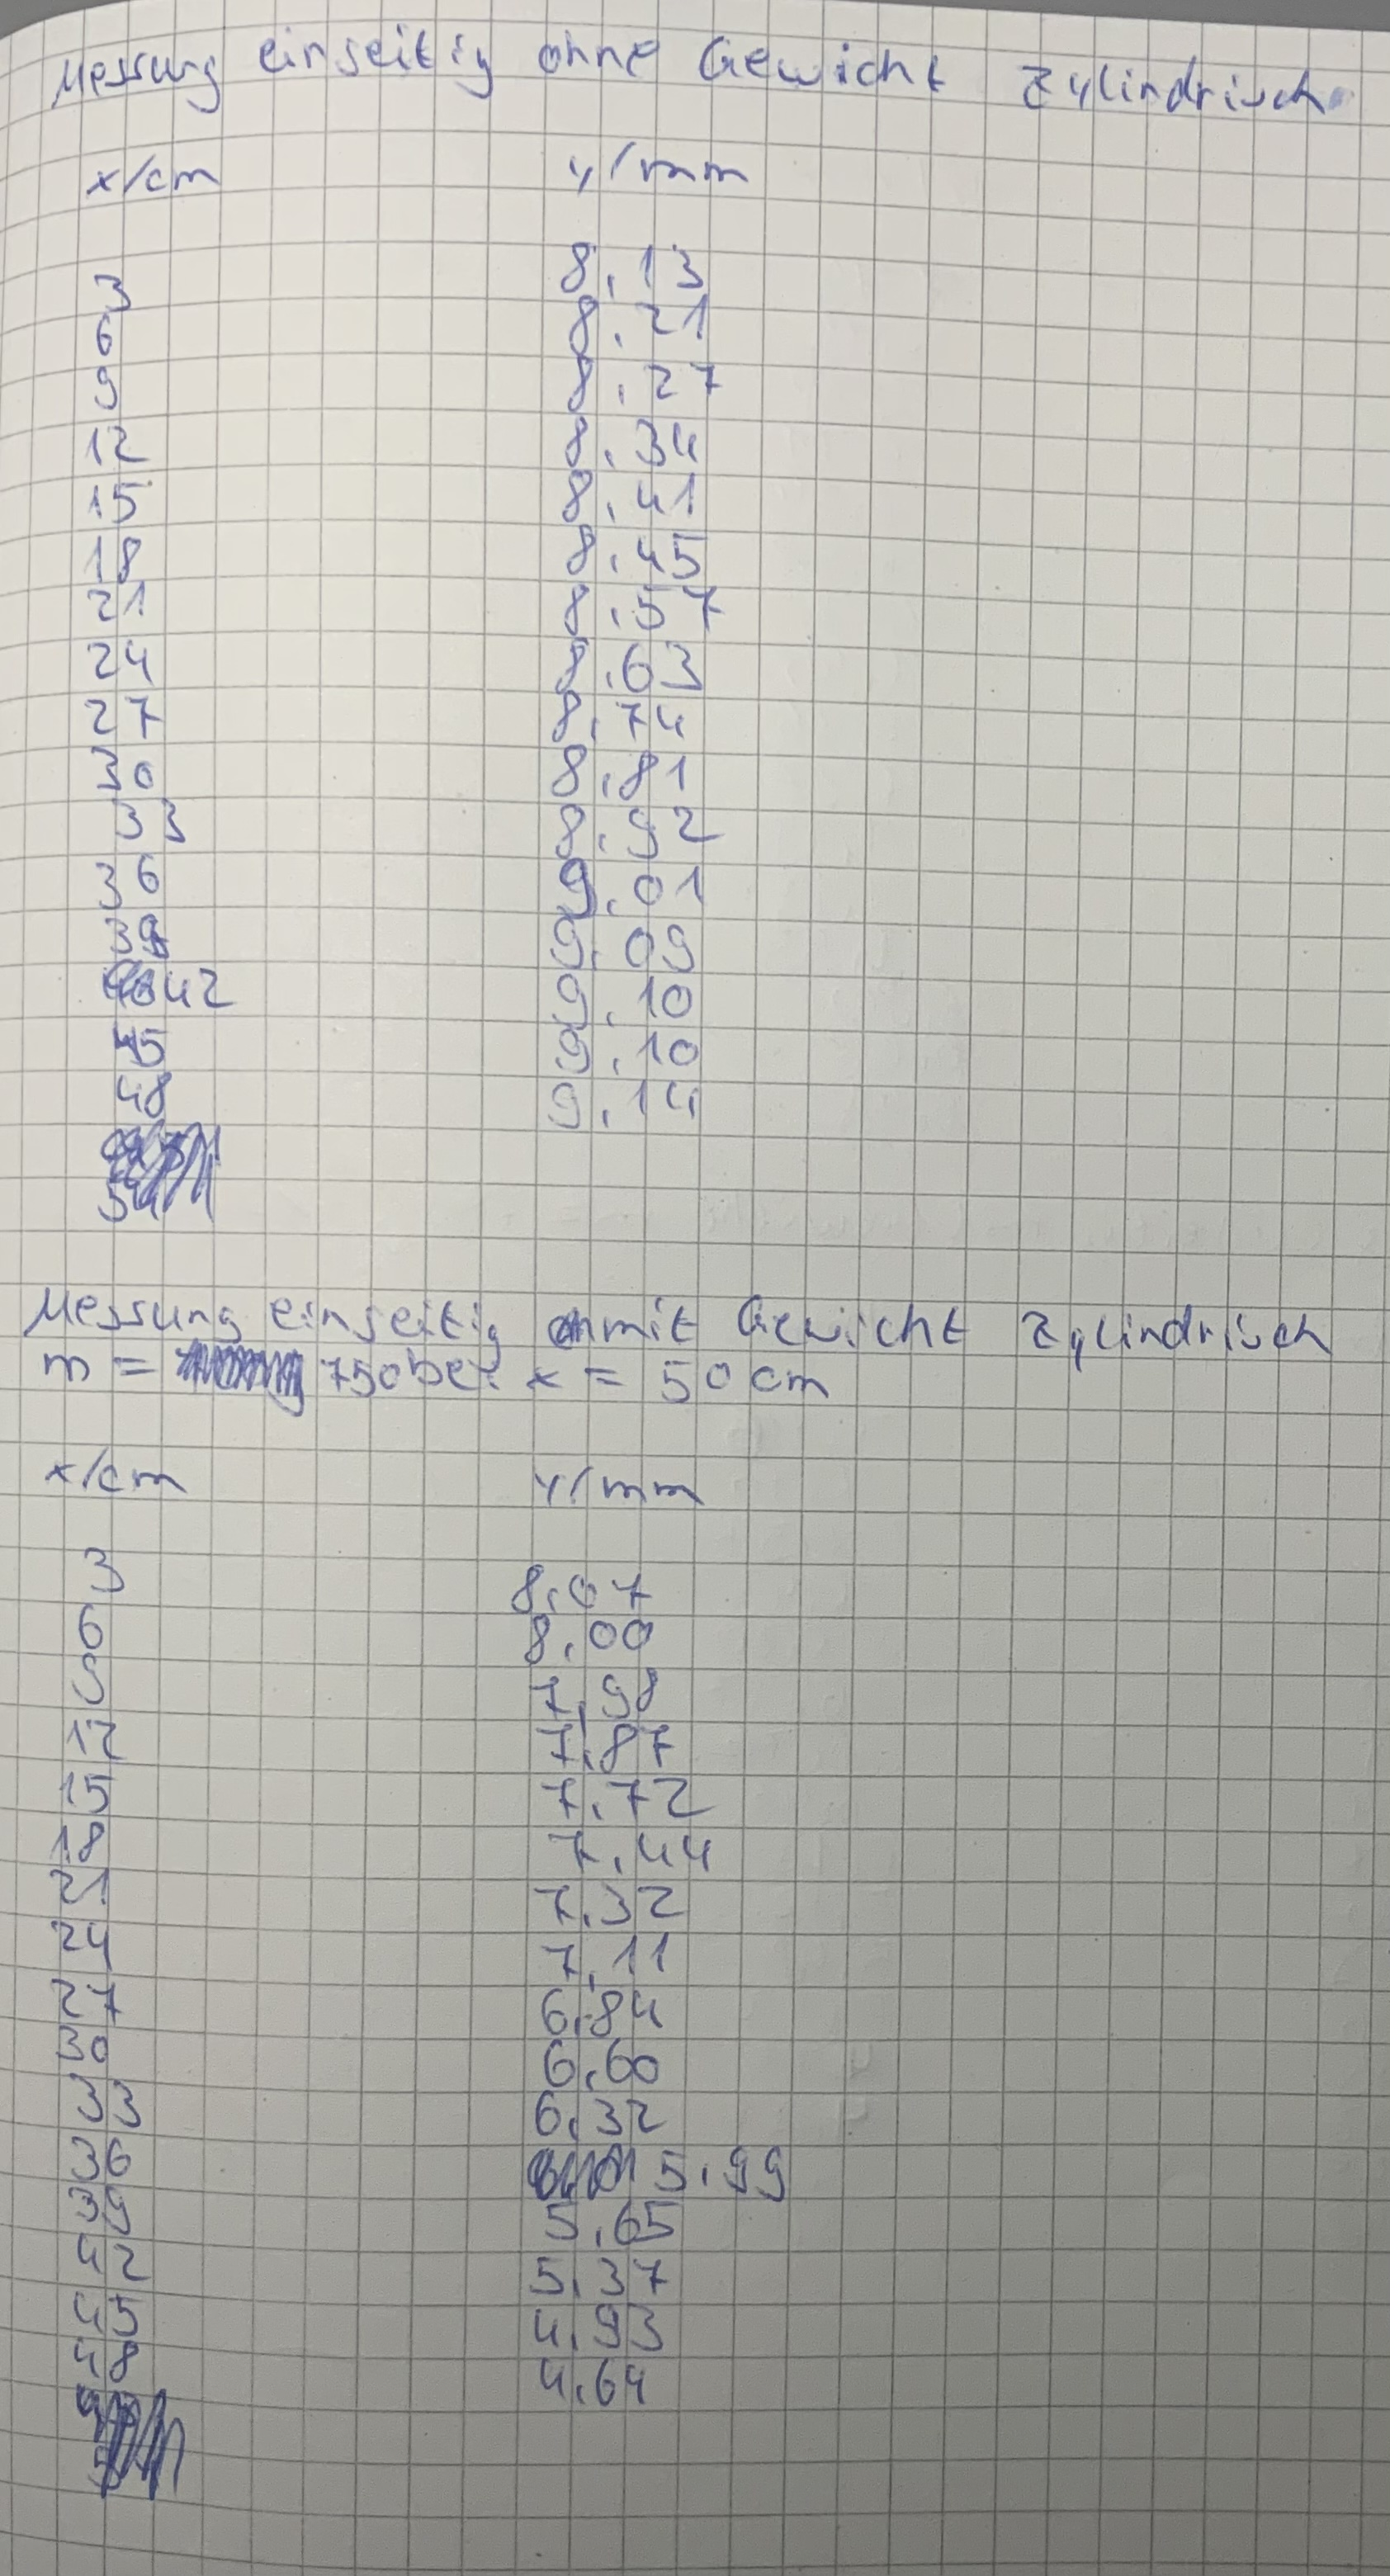
\includegraphics[width=0.75\textwidth]{Dateien/Bild4.jpeg}
    \caption{Originale Messdaten.}
    \label{fig:daten4}
\end{figure}